\documentclass[12pt]{article}

\usepackage[13643]{easymcm}  % Team control number
\usepackage{longtable}
\usepackage{booktabs}
\usepackage{algorithm}
\usepackage{algpseudocode}

\newcommand{\toB}[1]{\color{blue}#1\color{black}}

\problem{A}  % Problem number

\title{}  % Title

\begin{document}

\begin{abstract}

	\vspace{0.4cm}
	
	Dandelions, officially named \textit{Taraxacum officinale}, is know as an invasive species, which is likely to cause economic or environmental harm or harm to human health.
	
	\vspace{0.5cm}	
	In this paper, we design a \textbf{Dandelion Spread Model} by using Monte Carlo method.  
	
	Provided there is one dandelion at the edge of an open one-hectare plot of land, we need to predict the spread of dandelions over time.
	
	We input 3 groups of random variables to our model, i.e., temperature, wind and humidity.  Some details like equivalent temperature curve, dispersal distances under horizontal wind and updrafts, and random biological characteristics/behaviors are also taken into account.
	
	We output all the locations of dandelions that spread on the land over time.  In order to get stable results, we run the model with 2 phases and for each phase we run 1000 times.  In the first phase, we determine the optimal starting time and in the second phase, we fix the starting time and get the most probable outcome.
	
	We apply our model to 6 locations and conclude the statistic characteristics.  We also conduct a sensitivity analysis and discuss the strengths and weaknesses.
	
	\vspace{0.5cm}
	
	In this paper, we also devise a \textbf{Plant Impact Factor Model} to measure the impact of invasive plants on humans and the environment.  We define a global impact factor and a local impact factor for different purposes.
	
	We consider many attributes, including the plant's characteristics, its effects on humans and the environment, and its local adaptation, and use the Analytic Hierarchy Process to get the weights for each attribute.
	
	We apply our model to 226 invasive species and calculate their global impact factors.  We also choose 5 plants and calculate their local impact factors at 3 locations.
	
	We conduct a sensitivity analysis and discuss the strengths and weaknesses.
	
	\vspace{0.5cm}
	At the end of this paper, we write an article to elaborate on our viewpoint on invasive species.  Rather than think they are enemies, we need to learn how to get along with them.  To we human beings, they are just vigorous friends.
	
\end{abstract}

\maketitle
\tableofcontents

\section{Introduction}

	\subsection{Background}
	
	Dandelion is a very common plant with scientific name \textit{Taraxacum officinale}, which is stemless, lactiferous and perennial\autocite{stewart2002biology}.  We can find them at roadsides, in wild fields or at inconspicuous places.  Just imagine that these little herbs with beautiful yellow flowers have been evolving on this planet for about 30 million years\autocite{dandelionhistory} - even longer than we human beings!
	
	But currently they are labeled as an invasive plant.  \textbf{Invasive species} is a relative concept.  It means an alien species whose introduction does or is likely to cause economic or environmental harm or harm to human health\autocite{defInvasive}.  In some regions, dandelions do have some traits that make them invasive.  They can adapt different environments.  They have high growth rate and spread fast. They are likely to cuddle together and crowd out desirable plants, particularly in lawns.  Also, they have deep taproots that enable them to pull available water out of the soil.  It is also mentioned that dandelions could cause significant economic damage and infestation of other crops worldwide\autocite{stewart2002biology}.
	
	To disclose the reason that dandelion becomes invasive, researchers have done many studies on how the environment affects dandelion.  Laboratory and field studies have discussed the impact of climatic factors on its growth. Laboratory studies have been conducted on the relationship between germination rate and ambiances, such as light and temperature\autocite{letchamo1996light}.  Field studies have also been conducted on the same topic, providing credibility for the theoretical conclusions\autocite{yoneda1991effects}.  Studies have provided insights on the drought tolerance of dandelions\autocite{brock2005drought}. In the meanwhile, soil pollution and geographic factors are also being considered\autocite{verhoeven2013geographic}.
	
	Researchers have also paid great attention to dandelion dispersal, which is a major way for dandelion propagation.  Past papers have analyzed the structure of dandelion seeds and the effects of humidity on their structure, which affected the dispersal speed\autocite{greene1989model}. Scientists have modeled the aerodynamics of the seeds and demonstrated the effects of wind speed and directions.  It has also been proved that updrafts could not be neglected\autocite{tackenberg2003dandelion}.
	
	Beside this particular species, researchers have discussed invasive species more generally.  Ecologists have used species native to the invaded range as ``control species'' in attempting to determine the traits associated with invasive plant species\autocite{muth2006traits}.  A protocol has been developed for categorizing non-native plants according to their negative impacts on biodiversity in a large area such as a state, nation, or ecological region\autocite{randall2008invasive}.  Some online tools like \href{https://www.imapinvasives.org/decision-analysis-tool}{PIMDAT}\autocite{PIMDAT} have been provided to help people make strategic decisions about invasive species control projects.  Currently we also have Best Management Practices (BMPs) to prevent the introduction and spread of invasive species\autocite{BMP}.
	
	Public databases play an important role in the research of invasive species, especially for plants. By conferring to some database, we can find plant data to study biological attributes of the invasive species\autocite{USDA}.  Another database for tracking introduced species provides a baseline for effective modeling of species trends and interactions, geospatially and temporally\autocite{US-RIIS}.  US Government's Open Data provides a lot of data for current invasive plants\autocite{DATAGOV}.
	\newpage
	
	\subsection{Problem Restatement}

	In this paper, we will solve 2 problems.
	
	\textbf{For the first problem}, we will predict the spread of dandelions within a year (360 days).  Suppose that a dandelion in its dispersal period happens to be adjacent to an open one-hectare plot of land.  We need to create a mathematical model to describe how the dandelion will spread its seeds and how its offspring will scatter on the land.  And we will have to consider the effect of various climatic conditions, such as temperate, arid, and tropical climates, on dandelion growth.
	
	\textbf{For the second problem}, we will need to devise an ``impact factor'' for invasive species.  We will formulate a mathematical model to determine this factor and apply it to dandelions and some other invasive plants.  We also need to make sure the plants are invasive in the regions we choose.

\section{Dandelion Spread Model}

	\subsection{Assumptions and Justifications}
	
		\begin{enumerate}
			
			\item \textbf{The initial dandelion is at the midpoint of the left edge of a one-hectare square plot of land.  Seeds blown out of the area are neglected.}
			\vspace{-0.125in}
			\begin{description}
				\item[Justification:] According to the problem, the initial dandelion is adjacent to an open one-hectare plot of land. In order to acquire maximum spread effect, we set the plant in the middle of the left edge and make the right side our spread area. The seeds drifting to the left of the edge will be neglected. We may imagine a river or a forest is at the left side, so seeds cannot spread back to the area.
			\end{description}
			
			\item \textbf{The field is planar.}
			\vspace{-0.125in}
			\begin{description}
				\item[Justification:] We only consider the case of flat terrain.  This helps us limits the spread to two dimensions.  Flat terrain simplifies the calculation of dispersal distance since the wind can be at a constant height and the seed landing will not be affected by different topography.
			\end{description}
			
			\item \textbf{There are no other plants in the spread area.}
			\vspace{-0.125in}
			\begin{description}
				\item[Justification:] Considering other plants would add complicity to our model, for example, we need to collect data of those plants and study the competitive interactions between plants.  So simplification is necessary.
				
				More specifically, we assume that no other plants hinder the spread of dandelions, which means:
				
				\textbf{a.} Dandelion seeds are not intercepted by other plants;
				
				\textbf{b.} Dandelions do not have to compete with other plants.  
				
			\end{description}
			
			\item \textbf{Wind direction is uniformly distributed from 0$^\circ$ to 360$^\circ$.}
			\vspace{-0.125in}
			\begin{description}
				\item[Justification:] \label{assumption:wind} Wind speed and direction can be affected by different topography, especially near the land. At the height of dandelions, there could be vortices and updrafts that will greatly affect dispersal.  Though we can obtain wind data from meteorological stations, the data may not be accurate for a  small area. Therefore, we decided not to use the real-time wind direction data.
				
				Moreover, though wind rose maps provide the probabilities for each direction, without knowing the orientation of the edge, we cannot decide the relative wind direction to this area.  So we assume wind direction is uniformly distributed from 0$^\circ$ to 360$^\circ$. In this way, all directions have same odds and we can pin the dandelion on an arbitrary edge.
			\end{description}
			
			\item \textbf{Dandelion number always increases.}
			\vspace{-0.125in}
			\begin{description}
				\item[Justification:] More specifically, we assume that there are none of the followings:
				 
				 \textbf{a.} Human intervention;
				 
				 \textbf{b.} Natural enemies;
				 
				 \textbf{c.} Extreme weather conditions.
				
				This assumption simplifies our model.  Without considering above conditions, it will be an carefree place for dandelion growth.  And if we notice that the dandelion is a perennial herb, it is safe to assume the number will always increase .
			\end{description}
			
		\end{enumerate}
		
	
	

	
	\subsection{Model Overview}
		
		We will use a Monte Carlo simulation model to solve the problem.
		
		In reality, we find that sometimes dandelions grow in clusters, and at other times they are very sparse. Actually the spread process is affected by many random factors, including climate condition, wind speed and direction, topographical features and so on.  In order to eliminate this randomness, we need a method to find statistical patterns from repeating the process many times.  Candidates are neural network, deep learning, stochastic process, etc.  Among them, the Monte Carlo method becomes an option due to its simplicity.  Its underlying concept is to introduce randomness to solve problems.   It relies on repeated random sampling to obtain numerical results.  We will simulate dandelion spread process by going through the process many times, observing the results from a statistical perspective and drawing some conclusions.
		
		As the input for our model, we consider five environmental factors, as shown in Table \ref{tb:vars}.  
		
		{
			\fontsize{10}{14}\selectfont
			{
				\begin{longtable}{ccc}
					\caption{Environmental factors}
					\label{tb:vars}\\
					\toprule
					Symbol&Description&Unit\\
					\toprule
					$\mu_T$&Mean temperature&$^\circ$C\\
					$\sigma_T$&Standard deviation of temperature&$^\circ$C\\
					$\mu_W$&Mean wind speed&m/s\\
					$\sigma_W$&Standard deviation of wind speed&m/s\\
					$\mu_H$&Mean humidity&\%\\
					\bottomrule
				\end{longtable}
			}
		}
		
		And we will do the following steps to consider the environmental influence on the dandelion spread process:
		
		\begin{itemize}
			\vspace{-0.5cm}
			\item Construct a temperature curve in Section \ref{sec:temp}.  
			
			\vspace{-0.2cm}
			\item Model dispersal mechanisms in Section \ref{sec:wind}.
			
			\vspace{-0.2cm}
			\item Introduce an adaptation factor $k$ in Section \ref{sec:af}.  
		
		\end{itemize}
	
		\vspace{-0.5cm}
		Then our model will simulate the spread of dandelions by tracking every single dandelion according to a life cycle pattern, which we will model in Section \ref{sec:life}.  
		
		Next, we will choose 6 locations in the US.  For each location, we have one set of 5 input factors. We will run our model in 2 phases.  In the first phase, we will run 1000 times to get the optimal starting date for each location.  In the second phase, we will fix the starting date we get from the first phase and run another 1000 times to get the final ouput.
		
		We choose to run 1000 times because we find that the data with 1000 runs will exhibit an approximately normal distribution with a small margin of error for the mean.

		As the output of our model, we get all the dandelion locations for each day within 360 days.  
		
		In order to depict the statistical characteristics of dandelion spread, we conclude all the locations into 2 variables -- one is the \textbf{number} of dandelions and the other is the \textbf{mean distance} of dandelions from the initial one.  The first variable reflects spread intensity and the second one reflects spread range.


	
	\subsection{Temperature Curve}
	\label{sec:temp}
	
		\begin{wrapfigure}{r}{0.475\textwidth}
			\vspace{-0.4cm}
			\centering
			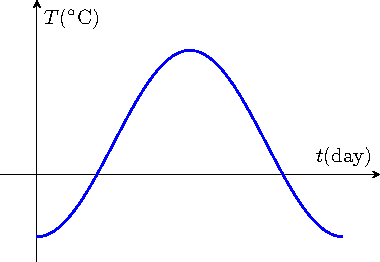
\includegraphics{fig-temperature_curve.pdf}
			\caption{Temperature curve}
			\label{fig:temp}
		\end{wrapfigure}
		
		We assume that the temperature follows a sinusoidal curve, as shown in Fig.\ref{fig:temp}.  We only consider locations in the northern hemisphere, so we further assume that the lowest temperature is reached on Jan.1st, when time $t = 0$.  We observe that the period of the curve is 360 (for convenience, we set each month to 30 days).  Thus, we write the equation as
		
		\[
			T = -A \cos{\frac{2\pi}{360} t} + B.
		\]
		
		These conditions should be satisfied:
		
		\[
			\mu_T = \frac1{360} \int_0^{360} (-A \cos{\frac{2\pi}{360} t} + B) \, \mathrm{d}t,
		\]
		
		\[
			\sigma_T^2 = \frac1{360} \int_0^{360} \left[ (-A \cos{\frac{2\pi}{360} t} + B) - \mu_T \right] ^2 	\mathrm{d}t.
		\]
		
		Solving for $A$ and $B$, we get
		
		\begin{equation} \label{eq:temp}
			T = -\sqrt2 \sigma_T \cos{\frac{2\pi}{360} t} + \mu_T.
		\end{equation}





	\subsection{Dispersal Mechanisms}
	\label{sec:wind}
		
		For the \textbf{direction} of seed dispersal, we assume that the seed always follows the direction of the wind, which is uniformly distributed from 0$^\circ$ to 360$^\circ$ according to Assumption \ref{assumption:wind}.  
		
		For the \textbf{distance} of seed dispersal, we consider two types of wind, horizontal wind and updraft\autocite{tackenberg2003dandelion} (see Fig.\ref{fig:dispersal}).  The seed travels either a normal distance $s_N$ due to horizontal wind or a long distance $s_L$ due to updraft.  We set dispersal \textbf{distance} as the greater one between $s_N$ and  $s_L$.
		
		\begin{figure}[htbp]
			\centering
			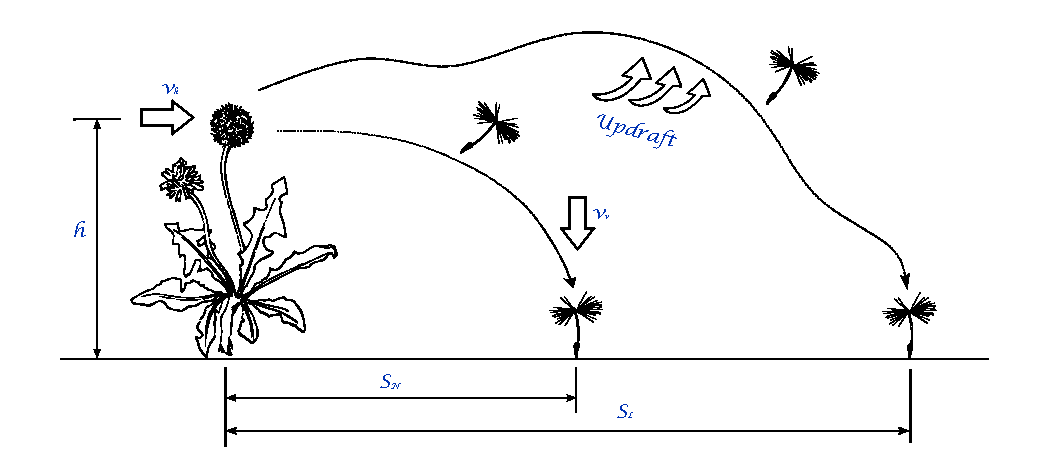
\includegraphics {wind_mode.pdf}
			\caption{Dandelion dispersal distance}
			\label{fig:dispersal}
		\end{figure}
		
		\subsubsection{Normal Distance $s_N$}
		
		In the case of horizontal wind, we have
		\begin{equation}\label{eq:hwind}
		 \frac{s_N}{v_h} = \frac{h}{v_v},
		\end{equation}
		where:
		
		$h$ is the height of the puffball, which is evaluated in Section \ref{sec:life};
		
		$v_v$ is the vertical component of the velocity of the seed, which is a constant value, 0.4 m/s\autocite{tackenberg2003dandelion}.
		
		$v_h$ is the speed of the horizontal wind, which follows a normal distribution with mean equals $\mu_W$ and standard deviation equals $\sigma_W$;

		\subsubsection{Long Distance $s_L$}
	
		\begin{wrapfigure}{r}{0.5\textwidth}
			\vspace{-1.5cm}
			\centering
			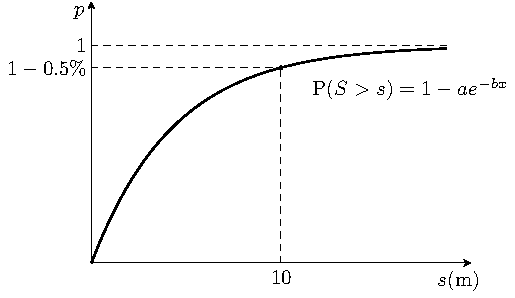
\includegraphics{fig-wind_curve.pdf}
			\caption{Cumulative distribution function of\\long-distance dispersal}
			\label{fig:longDistance}
		\end{wrapfigure}
		
		In the case of updraft, we suppose that $s_L$ follows an exponential distribution\autocite{okubo1989theoretical} with cumulative distribution function $\mathrm{P} (s_L < s) = 1 - ae^{-bs}$.  We know $\mathrm{P} (s_L < 0) = 0$.  We also know that the probability of a seed being blown further than 10 meters is 0.5\%\autocite{tackenberg2003dandelion}.  Therefore we can get
		
		\begin{equation}\label{eq:updraft}
			\mathrm{P} (s_L < s) = 1 - e^{-0.53 s}.
		\end{equation}
		
		\newpage
		\subsubsection{Dandelion Density}
		
		The leafs of dandelions have a radius of around 15cm.  If a seed lands without falling on the leaf of another dandelion, the dandelion density should be less than $(1/0.15)^2$ = 45 plants/m$^2$.  If a seed arrives at a location whose vicinity has a density greater than this maximum value, the seed fails to land, which means it is not counted in our model.
		
		
		
		
		
	\subsection{Adaptation Factor}
	\label{sec:af}
		
			We introduce an adaptation factor $k$ which is evaluated by using $T$ and $\mu_H$.  Dandelions prefer temperate climates and relatively high humidity.  We divide temperature into three ranks, which indicate if the temperature is suitable for the dandelion.  We also divide humidity into three ranks, which indicate if the humidity is suitable for the dandelion.  On a given day, we calculate $k$ by computing the arithmetic mean of the rank for temperature and humidity and scaling $k$ so that $0 \leq k \leq 1$.
			
			We use $k$ to determine the mean value of some parameters of dandelions, such as the height of the puffball.  To allow for some variation, we let the parameters follow normal distributions with
			\begin{equation}
				\begin{gathered}
					\mu_{\mathrm{parameter}} = \left( \mathrm{worst} + \frac{\mathrm{best} - \mathrm{worst}}4 \right) + k \frac{\mathrm{best} - \mathrm{worst}}2, \\
					\sigma_{\mathrm{parameter}} = \frac{\mathrm{best} - \mathrm{worst}}{12}.
				\end{gathered}
			\end{equation}
			The worst and best values for the relevant parameters will be given in Section \ref{sec:life}.  If the a parameter exceeds the limits, it is set to the limit.
		
		
		
		
		
	\subsection{Dandelion Life Cycle}
	\label{sec:life}
		
		A dandelion can transfer between 6 states: \textbf{seed}, \textbf{developing}, \textbf{dispersal}, \textbf{inter-dispersal}, \textbf{hold}, and \textbf{dormancy}.
		
		\begin{figure}[htbp]
			\centering
			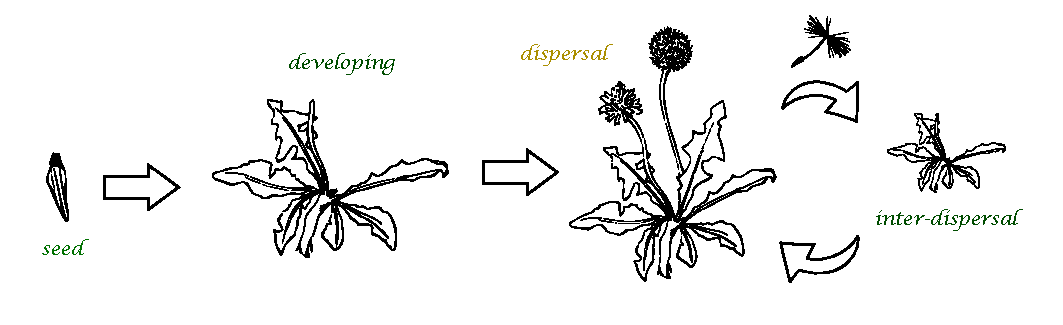
\includegraphics {life_cycle.pdf}
			\caption{Dandelion life cycle}
			\label{fig:lifeCycle}
		\end{figure}
		
		\begin{itemize}
			
			\item Out of all \textbf{seed}s, only 2\% will successfully germinate\autocite{honek2005post}.  These seeds will spend 3 days growing into the developing stage\autocite{stewart2002biology}.
			
			\item The \textbf{developing} stage is the time from sprouting to seed ripening.  It takes a sprout 60--95 days to grow into a flower, and an additional 9--12 days for the flower to ripen\autocite{gardenorganicNAripen}.  The exact duration of this stage is determined by the adaptation factor $k$ (worst = 107, best = 69) per Section \ref{sec:af}.
			
			\item The \textbf{dispersal} stage lasts 10 days.  A dandelion plant can produce around 10 seed heads per year and it usually flowers twice, so it produces 5 heads every time it flowers.  The number of seeds on each head is determined by $k$ (worst = 150, best = 200)\autocite{dukeNAdandelion}.  It takes each head 2 days to disperse its seeds.  The height of the puffball, $h$, is determined by $k$ (worst = 12, best = 40)\autocite{veggiegardenNAstem}.  The seeds are dispersed per the method stated in Section \ref{sec:wind}.
			
			\item The \textbf{inter-dispersal} stage is the stage between two dispersal stages of a plant.  In this stage, dandelions regrow their scapes and flowers.  Since most dandelions that flowered in spring usually flower again in fall\autocite{stewart2002biology}, the duration of this stage is set to be half a year, which is 180 days.   
			
		\end{itemize}
		We also consider two additional states, \textbf{hold} and \textbf{dormancy}.		
		\begin{itemize}
			
			\item When $T > 24^\circ$C, only 12.5\% of the flowers bloom and disperse their seeds\autocite{yoshie2020effects}.  We let dandelions enter dispersal by probability 12.5\% and move the rest into the \textbf{hold} stage.  In this stage, flowers are held in buds.  As soon as $T$ falls below $24^\circ$C, flowers can bloom and disperse seeds.  
		
			\item Dandelions enter the \textbf{dormancy} stage when $T < 0^\circ$C.  The temperature is low and it is likely that it snows.  All life activities of dandelions are paused.  As soon as $T$ rises above $0^\circ$C, dandelions resume the previous stage.
		
		\end{itemize}
		
		
		
		
		
	\subsection{Algorithm}
		\vspace{-0.4cm}
		{
			\fontsize{10}{14}\selectfont
			{
				\setlength{\parindent}{-1em}
				
				{
				\fontsize{12}{18}\selectfont
				\begin{longtable}{p{6.65in}}
					\toprule
					\textbf{Monte Carlo simulation algorithm for dandelion spread}\\
					\textbf{INPUT:} run times \toB{$n$ } and environment factors \toB{$\mu_T$}, \toB{$\sigma_T$}, \toB{$\mu_W$}, \toB{$\sigma_W$ } and \toB{$\mu_H$}\\
					\bottomrule
				\end{longtable}
				}
			
				\vspace{-0.5em}
				\begin{algorithmic}
					\For{1 to \toB{$n$}}
					\ForAll{\toB{$t$ } in days of one year}
					\State \toB{$T$ } $\gets$ evaluate current temperature per Eq.\ref{eq:temp}
					\State \toB{$k$ } $\gets$ evaluate adaptation factor per Section \ref{sec:af}
					\For{\toB{$dandelion$ } in current all dandelions}
					\State \textbf{if} \toB{$T$ } < 0 \textbf{then} \toB{$previous\,status$ } $\gets$ \toB{$current\,status$}, \toB{$current\,status$ } $\gets$ \textbf{Dormancy}
					\State \textbf{if} \toB{$current\,status$ } is \textbf{Dormancy} and \toB{$T$ } > 0 \textbf{then} \toB{$current\,status$ } $\gets$ \toB{$previous\,status$}
					\State \textbf{if} \toB{$current\,status$ } is \textbf{Hold} and \toB{$T$ } < 24 \textbf{then} \toB{$current\,status$ } $\gets$ \toB{$previous\,status$}
					
					\If{\toB{$current\,status$ } is \textbf{Developing} or \toB{$current\,status$ } is \textbf{Inter-dispersal}}
					\If{days of \toB{$current\,status$ } reaches the next stage}
					\If{\toB{$T$ } > 24}
					\State \toB{$current\,status$ } $\gets$ \textbf{Dispersal} with probability 0.125
					\If{\textbf{Dispersal} successfully}
					\State \toB{$current\,status$ } $\gets$ \textbf{Dispersal}
					\Else
					\State \toB{$previous\,status$ } $\gets$ \toB{$current\,status$}
					\State \toB{$current\,status$ } $\gets$ \textbf{Hold}
					\EndIf
					\Else
					\State \toB{$current\,status$ } $\gets$ \textbf{Dispersal}
					\EndIf
					\EndIf
					\EndIf
					
					\If{\toB{$current\,status$ } is \textbf{Seed}}
					\State \textbf{if} days of \toB{$current\,status$ } reaches the next stage \textbf{then} \toB{$current\,status$ } $\gets$ \textbf{Developing}
					\EndIf
					
					\If{\toB{$current\,status$ } is \textbf{Dispersal}}
					\State determine the seed count that needs to be dispersed
					\ForAll{\toB{$seed$ } in dispersing seeds}
					\State calculate dispersal distance per Section \ref{sec:wind}
					\State calculate land location and add it to \toB{$locations$ }
					\State generate a \toB{$new dandelion$ } with state \textbf{Seed}
					\EndFor
					\State \textbf{if} days of \toB{$current\,status$ } reaches the next stage \textbf{then} \toB{$current\,status$ } $\gets$ \textbf{Inter-dispersal}
					\EndIf
					
					
					\EndFor
					\EndFor
					\EndFor
					\State calculate \toB{$numbers$ } and \toB{$distances$ } per \toB{$locations$}
					\State \textbf{Return}{ \toB{$locations$ }, \toB{$numbers$ } and \toB{$distances$}}
				\end{algorithmic}
				
				{
				\fontsize{12}{18}\selectfont
				\begin{longtable}{p{6.6in}}
					\toprule
					\textbf{OUTPUT:} dandelion spread \toB{$locations$}, \toB{$numbers$ } and \toB{$mean\,distances$ } over days\\
					\bottomrule
				\end{longtable}
				}
			}
		}	
	
	\subsection{Dandelion Spread Results}
	
		\subsubsection{Location}
		
			We choose 6 locations in the US so that we have a variety of temperature and wind conditions.  AK is cold; CA, DC, and KS are warm; and FL and HI are relatively hot.  AK, DC, and KS have distinct seasons; CA and FL show moderate temperature fluctuations; and HI has very stable temperature.  The wind conditions also exhibit different patterns.  DC has notably large wind speed.  The values of the five environmental factors are listed in Table \ref{tb:locs}.  
			
			{
				\fontsize{10}{14}\selectfont
				{
					\begin{longtable}{ccccccc}
						\caption{Environmental factors for six locations}
						\label{tb:locs}\\
						\toprule
						State&Abbreviation&$\mu_T$ ($^\circ$C)&$\sigma_T$ ($^\circ$C)&$\mu_W$ (m/s)&$\sigma_W$ (m/s)&$\mu_H$ (\%)\\
						\toprule
						Alaska&AK&-0.05&9.08&7.27&1.42&81.46\\
						California&CA&16.20&4.99&6.02&0.90&80.36\\
						District of Columbia&DC&12.64&8.63&13.97&9.51&77.49\\
						Florida&FL&22.11&4.76&6.51&1.71&77.05\\
						Hawaii&HI&22.75&1.40&6.23&0.69&74.64\\
						Kansas&KS&12.58&9.98&8.58&1.55&79.37\\
						\bottomrule
					\end{longtable}
				}
			}
			\newpage
			
		\subsubsection{First Phase Results}	
			We run the model for 2 phases.
			
			In the first phase, we determine the optimal starting month of simulation.  For all 6 locations, we run the model with 12 cases that start respectively on the first day of each month, and get the number and mean distance for each case and each location.
			
			As an example, the results for Florida are shown in Fig.\ref{fig:start}.  The dandelion number varies greatly among the case, but the mean distance is approximately the same.  We can see that for Florida, we get the maximum dandelion number when the starting date is May 1st.  So we will use May as the starting month in the next phase.
			
			\begin{figure}[htbp]
				\centering
				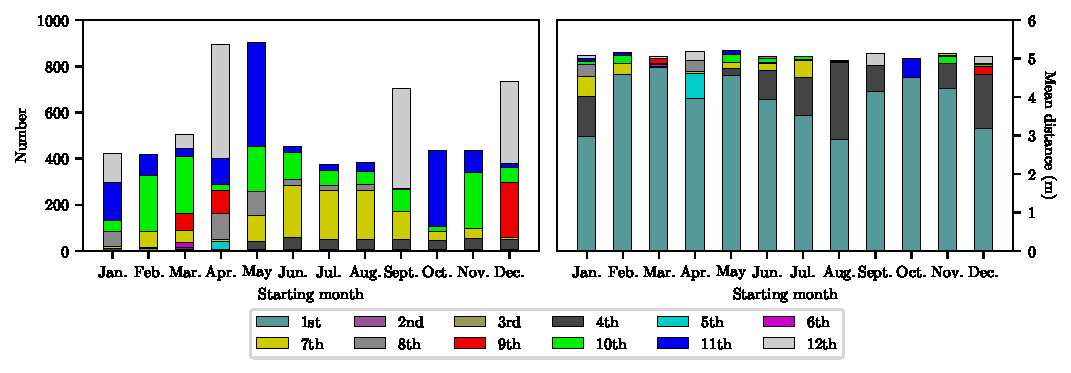
\includegraphics{start_month-number.pdf}
				\caption{Number and mean distance in Florida when simulation starts at different months}
				\label{fig:start}
			\end{figure}
			
			Table \ref{tb:start} lists all the data from the run of first phase.  The headers indicate the starting months, and the numbers in the table are the dandelion numbers at the end of 12 months.  The numbers corresponding to the optimal starting months are marked in blue.  In this way, we can determine that the optimal starting month is September for AK, August for CA, September for DC, May for FL, September for HI, and August for KS.
			
			{
				\fontsize{10}{14}\selectfont
				{
					\begin{longtable}{ccccccccccccc}
						\caption{Number at six locations when simulation starts at different dates}
						\label{tb:start}\\
						\toprule
						State&Jan.&Feb.&Mar.&Apr.&May&Jun.&Jul.&Aug.&Sept.&Oct.&Nov.&Dec.\\
						\toprule
						AK&74&79&70&35&44&75&43&49&\color{blue}\textbf{82}&72&74&75\\
						CA&547&567&545&532&585&561&544&\color{blue}\textbf{596}&564&566&581&563\\
						DC&1611&1589&1609&1563&1680&1657&1673&1733&\color{blue}\textbf{1808}&1696&1677&1658\\
						FL&424&417&505&895&\color{blue}\textbf{905}&453&375&384&706&436&435&736\\
						HI&519&329&610&593&586&596&308&543&\color{blue}\textbf{618}&383&385&600\\
						KS&823&276&268&405&548&274&266&\color{blue}\textbf{1067}&287&288&950&834\\
						\bottomrule
					\end{longtable}
				}
			}
			
			
			
		\subsubsection{Second Phase Results}
		
			In the second phase, we run the model 1000 times for each location beginning at the optimal starting month from the first phase.  The resulting frequency histogram for Florida is shown in Fig.\ref{fig:freqDand}.  We can see that both the number and the mean distance follow an approximately normal distribution.  
			
			\begin{figure}[htbp]
				\centering
				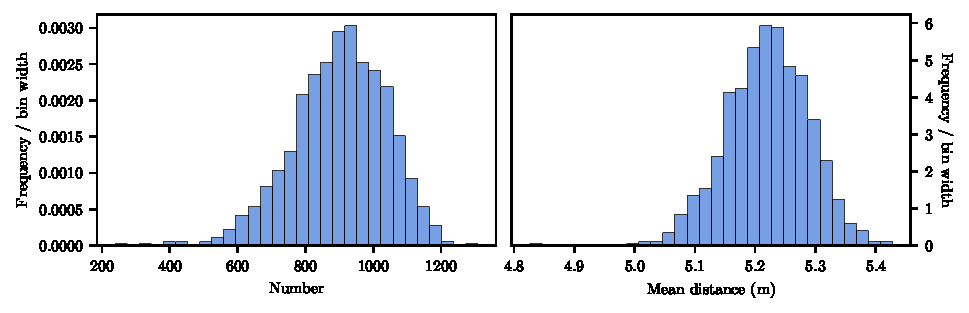
\includegraphics{number-frequency.pdf}
				\caption{Frequency distribution of number and mean distance in Florida}
				\label{fig:freqDand}
			\end{figure}
			
			We calculated several statistical characteristics for each location, as shown in Table \ref{tb:numDistribution} and Table \ref{tb:distDistribution}.	 We examine the statistics for dandelion number.  The confidence interval of the mean is relatively small for all locations, which implies the mean is quite accurate.  The standard deviation and range are large, which shows that the spread of dandelions is easily affected by random factors such as fluctuations in the environment.  For all locations except California, the distributions are platykurtic.  For all locations except Alaska, the distribution is skewed to the left.  Its mass is concentrated on the right, so the dandelion number is slightly more likely to be greater than the mean rather than smaller.  However, because of the unfavorable environmental conditions in Alaska, the number is more likely to be smaller than the mean.
			
			{
				\fontsize{10}{14}\selectfont
				{
					\begin{longtable}{cccccccc}
						\caption{Descriptive statistics of number at six locations}
						\label{tb:numDistribution}\\
						\toprule
						Location&Mean&Standard Deviation&Kurtosis&Skewness&Range&Median&Confidence Level (95.0\%)\\
						\toprule
						AK&72.7&26.5&-0.11&0.38&150&71&1.64\\
						CA&595.1&82.48&3.78&-1.32&744&609&5.11\\
						DC&1780&484.9&-0.04&-0.03&3274&1772.5&30.1\\
						FL&886.4&140.4&1.04&-0.72&981&905&8.71\\
						HI&607.5&81.9&1.12&-0.79&565&617&5.08\\
						KS&1066&186.4&1.05&-0.72&1403&1096&11.6\\
						\bottomrule
					\end{longtable}
					
				}
			}
			
			{
				\fontsize{10}{14}\selectfont
				{
					\begin{longtable}{cccccccc}
						\caption{Descriptive Statistics of the mean distance at six locations}
						\label{tb:distDistribution}\\
						\toprule
						Location&Mean&Standard Deviation&Kurtosis&Skewness&Range&Median&Confidence Level (95.0\%)\\
						\toprule
						AK&4.29&0.18&0.44&0.25&1.28&4.29&0.01\\
						CA&4.52&0.09&0.51&-0.53&0.67&4.52&0.01\\
						DC&11.84&0.21&1.5&-0.51&1.93&11.85&0.01\\
						FL&5.21&0.07&1.91&-0.64&0.66&5.21&0.00\\
						HI&4.99&0.08&0.138&-0.27&0.5&4.99&0.00\\
						KS&6.52&0.05&0.8&-0.36&0.44&6.52&0.00\\
						\bottomrule
					\end{longtable}
				}
			}
			
			Out of the 1000 runs, we select the run that has a dandelion number closest to the mean value.  The positions and current stages of the dandelions at the end of 12 months are shown in Fig.\ref{fig:scatter5loc}.  For all locations except the District of Columbia, most dandelions grow in a semicircular ring centered at the origin.  Alaska is apparently unsuitable for dandelions to spread.  In California, Hawaii, Florida, and Kansas, dandelions all spread to a moderate range.
			
			\begin{figure}[htbp]
				\centering
				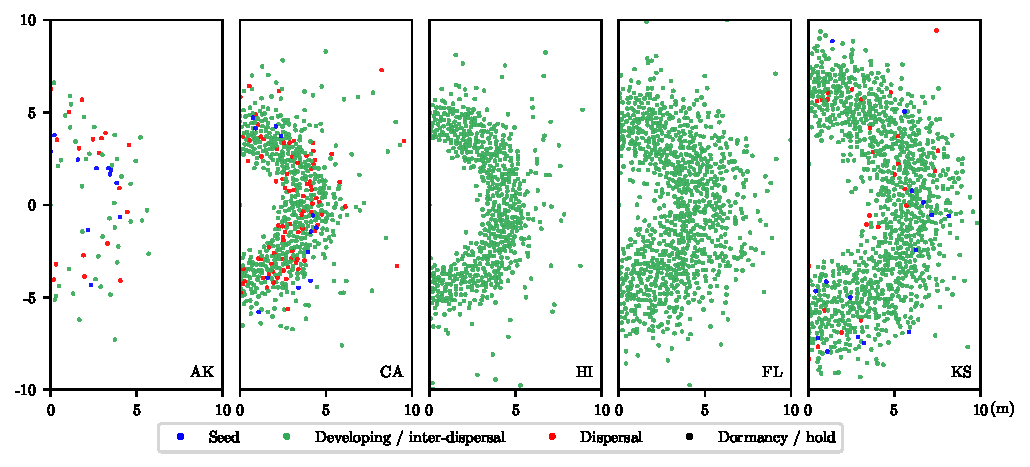
\includegraphics{spread_course-location_non_DC.pdf}
				\caption{The spread at the end of 12 months at different locations}
				\label{fig:scatter5loc}
				
				\vspace{1cm}

				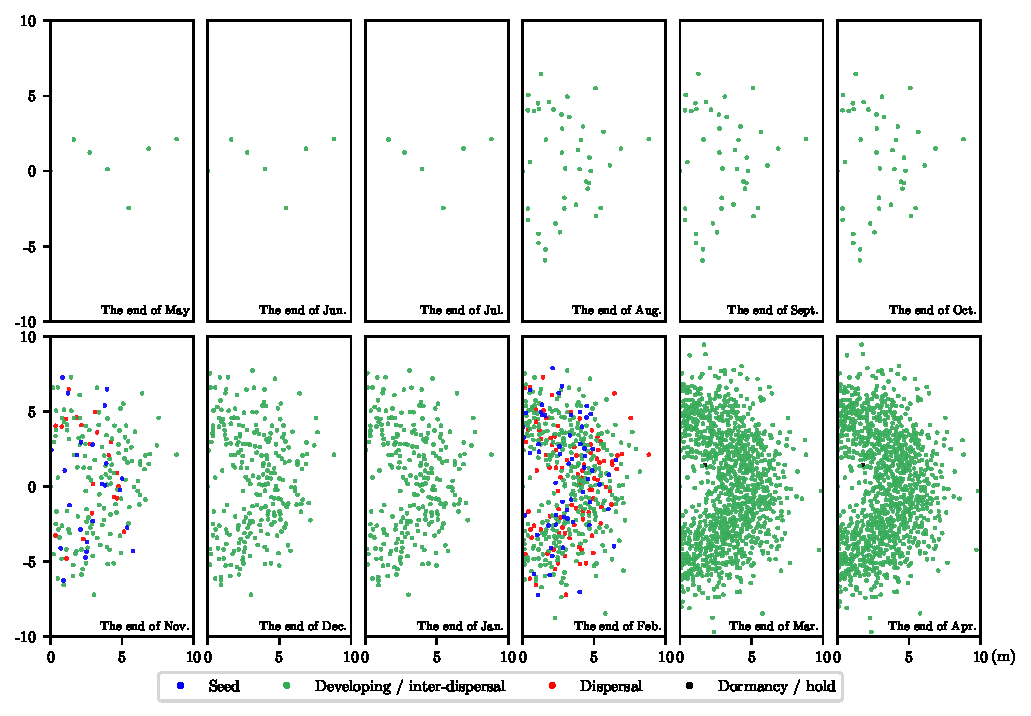
\includegraphics{spread_course-time.pdf}
				\caption{The spread during 12 months in the District of Columbia}
				\label{fig:spreadDC}
			\end{figure}
			\newpage
			
			District of Columbia has the most dandelions at the of 12 months.  We plotted dandelion spread at the end of each month this location (see Fig.\ref{fig:spreadDC}) so that it can be clearly seen how the dandelions spread in the course of time.  Compared to other locations, District of Columnbia has greater wind speed so the dandelions spread much further and they form a semicircle instead of a ring.  The closer to the origin, the denser the plants.  Additionally, there is a sudden increase every three months, which is caused by the flowering of a new generation of dandelions.
			
			Finally, we draw a graph of the natural logarithm of dandelion number in Fig.\ref{fig:time}.  The lines have several jumps and platforms.  The dandelion number increases exponentially at the end of each fixed period.  This conclusion coincides with our observation in Fig.\ref{fig:spreadDC}.  Again, Alaska is different.  Dandelions there are dormant in the first three months of the year, and eventually produce fewer offspring than other locations.
			
			\begin{figure}[htbp]
				\centering
				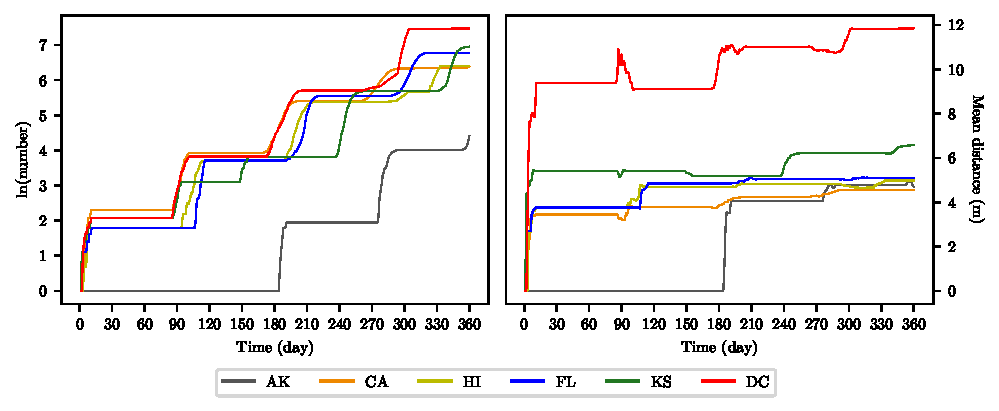
\includegraphics{number_mean_distance-time.pdf}
				\caption{Number and mean distance over time}
				\label{fig:time}
			\end{figure}
		
		
		
		\subsubsection{Sensitivity Analysis}
			
			We conduct a sensitivity analysis on the five factors from Table \ref{tb:vars} by varying one of them while keeping the other four fixed.  
			
			Fig.\ref{fig:saT} shows the results for temperature.  When $\mu_T$ falls below 7$^\circ$C or rises above 23$^\circ$C, dandelion number decreases sharply.  This is because dandelions are transferred to the dormancy or hold stages at certain temperatures.  The number is very sensitive to extreme temperatures, but only moderately sensitive to mild temperatures.  The mean distance increases with $\mu_T$ up to 19$^\circ$C, where the it temporarily levels off and begins to fall at 23$^\circ$C.  It has medium sensitivity to $\mu_T$.
			
			Both number and mean distance decreases as $\sigma_T$ increases.  They decrease relatively slowly below $\sigma_T = 5^\circ$C and rapidly above that value.  However, the overall sensitivity is not high for either number or mean distance.
			
			\begin{figure}[htbp]
				\centering
				\begin{minipage}{0.04\textwidth}\end{minipage}
				\begin{minipage}{0.46\textwidth}
					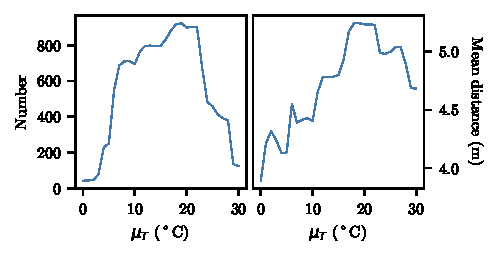
\includegraphics{sa_MuT.pdf}
				\end{minipage}
				\begin{minipage}{0.46\textwidth}
					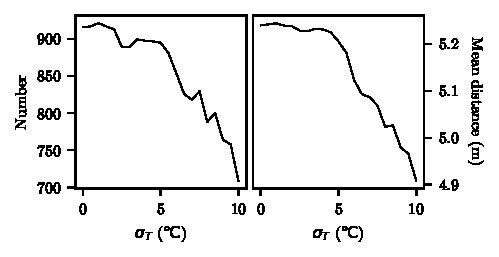
\includegraphics{sa_StdT.pdf}
				\end{minipage}
				\begin{minipage}{0.04\textwidth}\end{minipage}
				\caption{Sensitivity analysis: temperature}
				\label{fig:saT}
			\end{figure}
			
			Fig.\ref{fig:saW} shows the results for wind speed.  The number and mean distance have a positive correlation with $\mu_W$ and $\sigma_W$ and change drastically when the two factors vary.  When $\mu_W$ increases, seeds are dispersed farther and land further apart from each other.  When $\sigma_W$ increases, there is greater variation in dispersal distance.  In both cases it is less likely for seeds to land on other plants, making dandelion number rise quickly.
			
			\begin{figure}[htbp]
				\centering
				\begin{minipage}{0.04\textwidth}\end{minipage}
				\begin{minipage}{0.46\textwidth}
					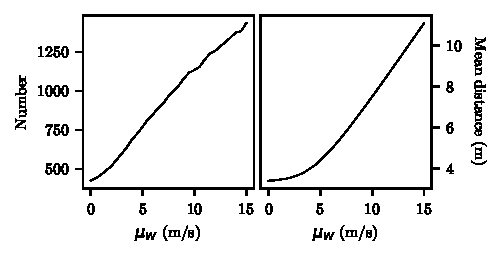
\includegraphics{sa_MuW.pdf}
				\end{minipage}
				\begin{minipage}{0.46\textwidth}
					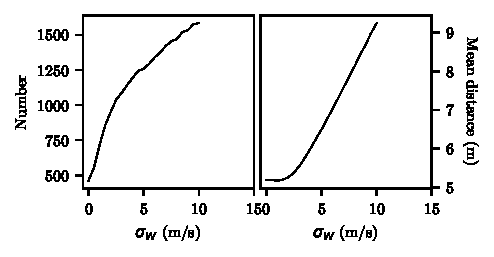
\includegraphics{sa_StdW.pdf}
				\end{minipage}
				\caption{Sensitivity analysis: wind speed}
				\label{fig:saW}
			\end{figure}
			
			Fig.\ref{fig:saH} shows the results for humidity.  There are three levels of number and mean distance corresponding to different humidity.  This is because of the three ranks for humidity that are used in the calculation of the adaptation factor $k$, see Section \ref{sec:af}.
			
			\begin{figure}[htbp]
				\centering
				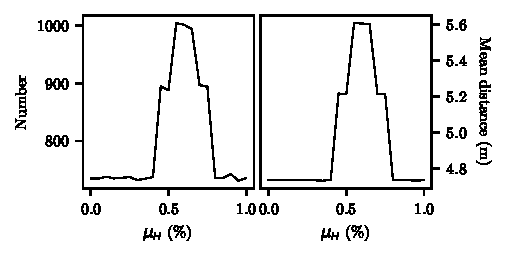
\includegraphics{sa_Hum.pdf}
				\caption{Sensitivity analysis: humidity}
				\label{fig:saH}
			\end{figure}
			
			
			
		\subsubsection{Strengths and Weaknesses}
		
			\paragraph{Strengths}
			\vspace{-0.1cm}
			\begin{itemize}
				\vspace{-0.3cm}
				\item Our model is \textbf{realistic}.  We used data for real locations.  And we considered how environmental factors and random variations contribute to dandelion spread.  Besides, we tracked every plant during the entire spread process.  
				
				\vspace{-0.3cm}
				\item Our model is \textbf{easy to understand and implement}.  The simulation method is very intuitive, and the model only requires five input values that are easily acquired from meteorological databases.
				
				\vspace{-0.3cm}
				\item Our model is \textbf{extensible}.  We can easily consider other factors by adding a component to the model.  For example, if we want to consider the effect of rain, we can determine the effects of rain on the different stages of dandelions and add this new component to our current model.
			\end{itemize}
			
			\paragraph{Weaknesses}
			\vspace{-0.5cm}
			\begin{itemize}
				\vspace{-0.3cm}
				\item Our model is \textbf{time-intensive}.  To get a fairly accurate result, we have to run about 1000 times for each location.  Compared to other possible models, the efficiency of our model is relatively low.
				
				\vspace{-0.3cm}
				\item The \textbf{adaptation factor} may be an over-simplification.  It may not represent the reality very accurately.  If we can acquire the relationship between dandelion parameters and climate conditions, we will be able to substitute the adaptation factor with some more accurate components.
				
				\vspace{-0.3cm}
				\item Our model \textbf{misses certain factors}.  We did not consider rain, which stops flowers from blooming and hinders seed dispersal.  Other missed factors include interactions with other plants and human intervention.  These can be added as new components in the future.
				
			\end{itemize}

		
		
		
		
\section{Plant Impact Factor Model}

	\subsection{Assumptions and Justifications}
	
		\begin{enumerate}
			
			\item \textbf{A plant's impact has a direct correlation with its biological characteristics.}
			\vspace{-0.125in}
			\begin{description}
				\item[Justification:] Study shows that the invasiveness of plant species is closely related to \\performance-related traits\autocite{van2010meta}.  Thus we can think of biological characteristics as fairly reliable indicators on the invasiveness, which is the plant's ability to cause harm to the environment and to humans.  
			\end{description}
			
			\item \label{assumption:offset} \textbf{A plant's impact can be mitigated by its benefits.}
			\vspace{-0.125in}
			\begin{description}
				\item[Justification:] If plants are edible for animals or beneficial for the environment in some other ways, it is likely that the environment will be subject to less harm overall.  Likewise, if plants can be made into products or utilized in other ways, they can benefit the economy and cause less harm to humans.  
			\end{description}
			
			\item \textbf{At locations with higher population density, the impact of a plant is greater.}
			\vspace{-0.125in}
			\begin{description}
				\item[Justification:] At places with higher population density, it is likely that people try harder to get rid of undesirable species.  This leads to more expenditure on the control of the species, which means the impact is greater.  At places with low population density, there is less human intervention. Non-native plants may reach an equilibrium with native ones, thus causing less impact.  
			\end{description}
			
		\end{enumerate}
	
	\subsection{Model Description}
	
	\subsubsection{Model Overview}
		
		The \textbf{impact factor} is a measure of adverse impact that an invasive plant can make on the environment and human beings.  
		
		We define two types of impact factors, namely \textbf{global impact factor} and \textbf{local impact factor}.  We also break down all the impact attributes into 3 categories.  \textbf{Category \textit{A}} is related to plant characteristics, \textbf{Category \textit{B}} is related to human and environment and \textbf{Category \textit{C}} is related to plant's local adaptation.  Global impact factor considers attributes from both \textbf{Category \textit{A}} and \textbf{Category \textit{B}}.  Local impact factor considers attributes from all 3 categories.
		
		With global impact factor, we can compare the invasiveness between species in general perspective.  For example, by using global impact factor, we can tell which one has more invasiveness between dandelion and clover, by and large.
		
		Local impact factor does more refined work.  By introducing more local adaptation attributes, we can tell the difference of invasiveness between locations for one species .  We can also compare the invasiveness for different species in different places.
		
		Table \ref{tb:syms} lists all the variables we will use in this model.
		
		{
			\fontsize{10}{14}\selectfont
			{
				\begin{longtable}{cc}
					
					\caption{Variable definition}
					\label{tb:syms}\\
					\toprule
					Symbol&Definition\\
					\toprule
					IF$_G$&Global impact factor\\
					IF$_L$&Local impact factor\\
					$\rho$&Invasion level coefficient\\
					$a_i$&Attribute value for $A_i$\\
					$b_j$&Attribute value for $B_j$\\
					$c_k$&Attribute value for $C_k$\\
					$\alpha_i$&The weight for attribute $A_i$\\
					$\beta_j$&The weight for attribute $B_j$\\
					$\gamma_k$&The weight for attribute $C_k$\\
					\bottomrule
					
				\end{longtable}
			}
		}
		The formulas for calculating global impact factor and local impact factor are as follows:
		\begin{equation} \label{eq:ifg}
			\mathrm{IF}_G = 100\rho \left( \sum_{} \alpha_ia_i + \sum_{} \beta_jb_j \right),
		\end{equation} 
		\begin{equation} \label{eq:ifl}
			\mathrm{IF}_L = 100\rho \left( \sum_{} \alpha_ia_i + \sum_{} \beta_jb_j + \sum_{} \gamma_kc_k \right).
		\end{equation}
		
		{
		
		\begin{itemize}
		\vspace{-0.2cm}
		\item \textbf{Invasion level coefficient $\rho$} is 0.9 if a plant is less widespread invasive, otherwise 1.0.
		\vspace{-0.2cm}
		\item \textbf{Attribute values} $a_i$, $b_j$ and $c_k$ are determined per Section \ref{sec:attr_value}.
		\vspace{-0.2cm}
		\item \textbf{Attribute weights} $\alpha_i$, $\beta_j$ and $\gamma_k$ are determined per Section \ref{sec:attr_weight}.
		\end{itemize}
		}
	
		\subsubsection{Attribute values}
		\label{sec:attr_value}
		
		Every attribute contains a list of options described in words than in numbers.  In order to leverage Eq.\ref{eq:ifg} and Eq.\ref{eq:ifl}, we need to map the options from words to numbers per Table \ref{tb:attributes}.
		\newpage
		{
			\fontsize{10}{14}\selectfont
			{
			\begin{longtable}{p{0.2in}p{1.5in}p{4.3in}}
				
				\caption{Attributes values}
				\label{tb:attributes}\\
				
				\toprule
				\multicolumn{1}{c}{\textbf{Symbol}} 
					& \multicolumn{1}{c}{\textbf{Attributes}}
					& \multicolumn{1}{c}{\textbf{$a_i$, $b_i$ and $c_i$ Evaluation}} \\
			
				\toprule
				\multicolumn{3}{l}{Category \textit{A} - Plant Characteristics}\\
				\midrule
				
				$A_1$ & Duration & $a_1=0.5$ (Annual), $0.75$ (Biennial), $1$ (Perennial)\\
				$A_2$ & Growing Habit & $a_2=0$ (Tree), $0.25$ (Shrub), $0.5$ (Vine), $0.75$ (Graminoid), $1$ (Forb/herb)\\ 
				$A_3$ & Growth Rate & The growth rate after successful establishment.\\
					&& $a_3=0.5$ (Slow), $0.75$ (Moderate), $1$ (Rapid)\\
				$A_4$ & Lifespan & $a_4=0.25$ (when $a_1=0.5$ or $0.75$), $0.5$ (Short), $0.75$ (Moderate), $1$ (Long) \\
				$A_5$ & Fertility Requirement & Relative level of nutrition (N, P, K) required for normal growth and development.\\
					 && $a_5=0.5$ (Low), $0.75$ (Medium), $1$ (High)\\
				$A_6$ & Fruit/Seed Abundance & The amount of seed produced.\\
					&& $a_6=0.25$ (None), $0.5$ (Low), $0.75$ (Medium), $1$ (High)\\
				$A_7$ & Propagated Methods & The propagation methods number, $n_7$. The methods can be Propagated by Bare Root, by Bulb, by Container, by Corm, by Cuttings, by Seed, by Sod, by Sprigs, or by Tubers. \\
					&& $a_7=0.25$ ($n_7=1$), $0.5$ ($n_7=2$), $0.75$ ($n_7=3$), $1$ ($n_7\geq4$)\\
				$A_8$ & Seed Spread Rate & The capability of the plant to spread through its seed production.\\
					&& $a_8=0.25$ (None), $0.5$ (Slow), $0.75$ (Moderate), $1$ (Rapid)\\
				$A_9$ & Seedling Vigor & The expected seedling survival percentage of the plant.\\
					&& $a_9=0.5$ (Low), $0.75$ (Medium), $1$ (High)\\
				
				\midrule
				\multicolumn{3}{l}{Category \textit{B} - Human and Environment}  \\
				\midrule
				
				$B_1$ & Toxicity & The relative toxicity of the plant to either humans or livestock.\\
					&& $b_1=0$ (None), $0.5$ (Slight), $0.75$ (Moderate), $1$ (Severe)\\
				$B_2$ & Product & The level of the plant known to be suitable for multiple types of products.\\
					&& $b_2=0$ (Copiousness), $0.25$ (Many), $0.5$ (Some), $0.75$ (few), $1$ (None)\\
				$B_3$ & Palatable Animal & The relative palatability of this plant to browsing animals or to grazing animals.\\
					&& $b_3=0$ (High), $0.5$ (Moderate), $0.75$ (Low), $1$ (None)\\
				$B_4$ & Palatable Human & The plant produce berries, nuts, seeds, or fruits are palatable to humans. \\
					&& $b_4=0.5$ (Yes), $1$ (No)\\
				$B_5$ & Commercial Availability & The plant propagules are in the commercial marketplace. \\
					&& $b_5=0.5$ (Yes), $1$ (No)\\
			
				\midrule
				\multicolumn{3}{l}{Category \textit{C} - Location}  \\
				\midrule
				
				$C_1$ & Soil Adaptation & The soil adaptation level.\\
				&& $c_1=0$ (Low), $0.5$ (Medium), $1$ (High)\\
				$C_2$ & Temperature Adaptation & The temperature adaptation level.\\
				&& $c_2=0$ (Low), $0.5$ (Medium), $1$ (High)\\
				$C_3$ & Humid Adaptation & The humid adaptation level.\\
				&& $c_3=0$ (Low), $0.5$ (Medium), $1$ (High)\\
				$C_4$ & Population Density & The level of population density.\\
				&& $c_4=0$ (Low), $0.5$ (Medium), $1$ (High)\\
			
				\bottomrule
			
			\end{longtable}
			}
		}
		\newpage
		
		Attributes $B_2$ (Product), $B_3$ (Palatable Animal), $B_4$ (Palatable Human), and $B_5$ (Commercial Availability) are special since they measure benefits rather than harms.  Per Assumption \ref{assumption:offset}, the greater the benefit, the less the impact.  Therefore, when the palatability is higher, or when the plant has more uses, the corresponding values are smaller.
		
		\subsubsection{Attribute weights}
		\label{sec:attr_weight}
		
		We use the Analytic Hierarchy Process (AHP) to obtain the weight vector.  When it is not easy to construct a weight vector by conferring to research papers, AHP is an option.  Since it makes pairwise comparisons and has a method to evaluate the rationality for those comparisons, it can reach a relatively reasonable result.
		
		We make comparisons between attributes according to Saaty's fundamental scale of absolute numbers\autocite{AHP}.  When two attributes are equally important, we get 1; when one attribute is moderately more important than the other, we get 3; when one attribute is strongly more important than the other, we get 5; when one attribute is much strongly more important than the other, we get 7; when one attribute is extremely more important than the other, we get 9.  Number 2, 4, 6 and 8 are used to express intermediate values.  
		
		The resulting comparison matrix is shown in Table \ref{tb:mat}.
		
		{
			\fontsize{10}{18}\selectfont
			{
				\begin{longtable}{c|ccccccccc|ccccc||cccc}
					
					\caption{AHP comparison matrix}
					\label{tb:mat}\\
					
					\toprule
					&$A_1$&$A_2$&$A_3$&$A_4$&$A_5$&$A_6$&$A_7$&$A_8$&$A_9$&$B_1$&$B_2$&$B_3$&$B_4$&$B_5$&$C_1$&$C_2$&$C_3$&$C_4$\\
					\toprule
					$A_1$&$1$&$1/3$&$1/7$&$1/3$&$1$&$1/7$&$1/4$&$1/7$&$1/5$&$1/9$&$1/5$&$1/3$&$1/4$&$1/4$&$1/5$&$1/5$&$1/5$&$1/3$\\
					$A_2$&$3$&$1$&$1/5$&$1$&$3$&$1/5$&$1/2$&$1/5$&$1/3$&$1/7$&$1/3$&$1$&$1/2$&$1/2$&$1/3$&$1/3$&$1/3$&$1$\\
					$A_3$&$7$&$5$&$1$&$5$&$7$&$1$&$4$&$1$&$3$&$1/3$&$3$&$5$&$4$&$4$&$3$&$3$&$3$&$5$\\
					$A_4$&$3$&$1$&$1/5$&$1$&$3$&$1/5$&$1/2$&$1/5$&$1/3$&$1/7$&$1/3$&$1$&$1/2$&$1/2$&$1/3$&$1/3$&$1/3$&$1$\\
					$A_5$&$1$&$1/3$&$1/7$&$1/3$&$1$&$1/7$&$1/4$&$1/7$&$1/5$&$1/9$&$1/5$&$1/3$&$1/4$&$1/4$&$1/5$&$1/5$&$1/5$&$1/3$\\
					$A_6$&$7$&$5$&$1$&$5$&$7$&$1$&$4$&$1$&$3$&$1/3$&$3$&$5$&$4$&$4$&$3$&$3$&$3$&$5$\\
					$A_7$&$4$&$2$&$1/4$&$2$&$4$&$1/4$&$1$&$1/4$&$1/2$&$1/4$&$1/2$&$2$&$1$&$1$&$1/2$&$1/2$&$1/2$&$2$\\
					$A_8$&$7$&$5$&$1$&$5$&$7$&$1$&$4$&$1$&$3$&$1/3$&$3$&$5$&$4$&$4$&$3$&$3$&$3$&$5$\\
					$A_9$&$5$&$3$&$1/3$&$3$&$5$&$1/3$&$2$&$1/3$&$1$&$1/5$&$1$&$3$&$2$&$2$&$1$&$1$&$1$&$3$\\
					\midrule
					$B_1$&$9$&$7$&$3$&$7$&$7$&$3$&$4$&$3$&$5$&$1$&$5$&$7$&$4$&$4$&$5$&$5$&$5$&$7$\\
					$B_2$&$5$&$3$&$1/3$&$3$&$5$&$1/3$&$2$&$1/3$&$1$&$1/5$&$1$&$3$&$2$&$2$&$1$&$1$&$1$&$3$\\
					$B_3$&$3$&$1$&$1/5$&$1$&$3$&$1/5$&$1/2$&$1/5$&$1/3$&$1/7$&$1/3$&$1$&$1/2$&$1/2$&$1/3$&$1/3$&$1/3$&$1$\\
					$B_4$&$4$&$2$&$1/4$&$2$&$4$&$1/4$&$1$&$1/4$&$1/2$&$1/4$&$1/2$&$2$&$1$&$1$&$1/2$&$1/2$&$1/2$&$2$\\
					$B_5$&$4$&$2$&$1/4$&$2$&$4$&$1/4$&$1$&$1/4$&$1/2$&$1/4$&$1/2$&$2$&$1$&$1$&$1/2$&$1/2$&$1/2$&$2$\\
					\midrule
					\midrule
					$C_1$&$5$&$3$&$1/3$&$3$&$5$&$1/3$&$2$&$1/3$&$1$&$1/5$&$1$&$3$&$2$&$2$&$1$&$1$&$1$&$3$\\
					$C_2$&$5$&$3$&$1/3$&$3$&$5$&$1/3$&$2$&$1/3$&$1$&$1/5$&$1$&$3$&$2$&$2$&$1$&$1$&$1$&$3$\\
					$C_3$&$5$&$3$&$1/3$&$3$&$5$&$1/3$&$2$&$1/3$&$1$&$1/5$&$1$&$3$&$2$&$2$&$1$&$1$&$1$&$3$\\
					$C_4$&$3$&$1$&$1/5$&$1$&$3$&$1/5$&$1/2$&$1/5$&$1/3$&$1/7$&$1/3$&$1$&$1/2$&$1/2$&$1/3$&$1/3$&$1/3$&$1$\\
					\bottomrule
				\end{longtable}
			}
		}	
		
		Note that attribute $B_1$ (Toxicity) is a predominant attribute in our model.  Toxic plants can poison the local environment and lead to a large expenditure for humans to control them.  Attributes $A_3$ (Growth Rate), $A_6$ (Fruit/Seed Abundance), $A_8$ (Seed Spread Rate) are also important because they  determine the spread rate of a plant when it is introduced to a new place.
		
		For the global impact factor, the comparison matrix is comprised of the numbers from first 14 rows and first 14 columns.  For the local impact factor, the comparison matrix is comprised of all the numbers in the table.  
		
		We conduct a consistency test on the global matrix and the local one.  The resulting CR is small enough for both matrices, so both matrices pass the test.
		
		{
			\fontsize{10}{14}\selectfont
			{
				\begin{longtable}{cccccccc}
					\caption{Consistency test}
					\label{tb:consistency}\\
					
					\toprule
					Impact Factor&Attribute Number&Max Eigenvalue 
					&\multirow{2}{*}{$\mathrm{CI}=\displaystyle \frac{\lambda_{max}-n}{n-1}$}
					&\multirow{2}{*}{$\mathrm{RI}$}
					&\multirow{2}{*}{$\mathrm{CR}=\displaystyle \frac{\mathrm{CI}}{\mathrm{RI}}$}
					&\multirow{2}{*}{$\mathrm{CR}<0.1?$}\\
					Type&$n$&$\lambda_{max}$\\
					\toprule
					Global&$14$&$14.501$&$0.0386$&$1.49$&0.0259&Yes\\
					Local&$18$&$18.561$&$0.0330$&$1.49$&0.0221&Yes\\
					\bottomrule
				\end{longtable}
			}
		}	
		
		For each matrix, we normalize the columns so that each column adds up to 1.  Then, we calculate the sum of each row to get a sum vector.  Last, we divide the sum vector by $n$ (the attribute number in Table \ref{tb:consistency}) to get the final weight vector.  
		
		The weight results are shown in Table \ref{tb:weights}.
	
		{
			\fontsize{10}{14}\selectfont
			{
				\begin{longtable}{c|ccccccccc}
					\caption{Weights results}
					\label{tb:weights}\\
					
					\toprule
					Type&$\alpha_1$&$\alpha_2$&$\alpha_3$&$\alpha_4$&$\alpha_5$&$\alpha_6$&$\alpha_7$&$\alpha_8$&$\alpha_9$\\
					\toprule
					Global&0.014&0.027&0.134&0.027&0.014&0.134&0.044&0.134&0.066\\
					Local&0.011&0.021&0.113&0.021&0.011&0.113&0.034&0.113&0.052\\
					\toprule
					\toprule
					&$\beta_1$&$\beta_2$&$\beta_3$&$\beta_4$&$\beta_5$&$\gamma_1$&$\gamma_2$&$\gamma_3$&$\gamma_4$\\
					\toprule
					Global&0.227&0.066&0.027&0.044&0.044&-&-&-&-\\
					Local&0.192&0.052&0.021&0.034&0.034&0.052&0.052&0.052&0.021\\
					\bottomrule
				\end{longtable}
			}
		}	
	
		\subsubsection{Algorithm}	
		\vspace{-0.4cm}
		{
			\fontsize{10}{14}\selectfont
			{
				\setlength{\parindent}{-1em}
				
				{
					\fontsize{12}{18}\selectfont
					\begin{longtable}{p{6.65in}}
						\toprule
						\textbf{Analytic Hierarchy Process Model for Impact Factor}\\
						\textbf{INPUT:} All the attribute options and \textbf{Invasive level coefficient $\rho$} \\
						\bottomrule
					\end{longtable}
				}
				
				\vspace{-0.5em}
				\begin{algorithmic}
					\State \toB{$global\,value\,vector$ } $\gets$ evaluate all the \textbf{Attribute values} from inputted attribute options per Table \ref{tb:attributes}
					\State \toB{$local\,value\,vector$ } $\gets$ evaluate all the \textbf{Attribute values} from inputted attribute options  per Table \ref{tb:attributes}
					\State \toB{$global\,weight\,vector$ } $\gets$ Table \ref{tb:weights}
					\State \toB{$local\,weight\,vector$ } $\gets$ Table \ref{tb:weights}
					\State \toB{IF$_G$ } $\gets$ \toB{$100\rho$ } times the dot product of \toB{$global\,value\,vector$ } and \toB{$global\,weight\,vector$ }
					\State \toB{IF$_L$ } $\gets$ \toB{$100\rho$ } times the dot product of \toB{$local\,value\,vector$ } and \toB{$local\,weight\,vector$ }
				\end{algorithmic}
				
				{
					\fontsize{12}{18}\selectfont
					\begin{longtable}{p{6.6in}}
						\toprule
						\textbf{OUTPUT:} \toB{IF$_G$ } and \toB{IF$_L$}\\
						\bottomrule
					\end{longtable}
				}
			}
		}	
		
	\subsection{Results}
	\subsubsection{Global Impact Factor Results}
		
		We downloaded a database containing a list of invasive plants from \href{https://www.sciencebase.gov/catalog/item/5b911a5ce4b0702d0e808588}{US-RIIS}\autocite{US-RIIS} and chose 226 plants from it.  These plants belong to 3 classes, 26 orders and 53 families.
		
		In order to get all the plant attributes, we developed a web crawler to grab data from \href{https://plants.usda.gov/home/}{USDA Plants Database}\autocite{USDA}.  Thus, we have all the attribute options ready for each plant.
		
		Then we implement this model to calculate the global impact factors for all 226 plants and rank them according to the factor.  Table \ref{tb:ranks} shows some results.
		
		{
			\fontsize{10}{14}\selectfont
			{
				\begin{longtable}{cccccc}
					\caption{Plant Rankings}
					\label{tb:ranks}\\
					
					\toprule
					Rank&Scientific Name&Vernacular Name&Duration&Growing Habit&IF$_G$\\
					\toprule
					1&\textit{Melilotus officinalis}&Sweetclover&Perennial&Forb/herb&84.5\\
					2&\textit{Senecio vulgaris}&Old-man-in-the-spring&Biennial&Forb/herb&83.3\\
					3&\textit{Ailanthus altissima}&Tree of heaven&Perennial&Tree&81.8\\
					4&\textit{Crotalaria spectabilis}&Showy rattlebox&Annual&Forb/herb&81.7\\
					5&\textit{Ranunculus repens}&Creeping buttercup&Perennial&Forb/herb&80.8\\
					6&\textit{Melilotus indicus}&Annual yellow sweetclover&Annual&Forb/herb&80.0\\
					7&\textit{Digitalis purpurea}&Purple foxglove&Biennial&Forb/herb&79.9\\
					8&\textit{Sorghum halepense}&Johnsongrass&Perennial&Graminoid&78.9\\
					9&\textit{Schedonorus arundinaceus}&Tall fescue&Perennial&Graminoid&76.8\\
					10&\textit{Vicia sativa}&Garden vetch&Annual&Forb/herb&73.8\\
					$\vdots$\\
					26&\textit{Taraxacum officinale}&Common dandelion&Perennial&Forb/herb&66.9\\
					\bottomrule
				\end{longtable}
			}
		}
		
		We observe that half of the top-10 plants are perennials and 7 of them are forbs/herbs.  Intriguingly, the tree of heaven, which is a tree, has made it to the third place.  This is mostly because it is toxic and grows rapidly. 
		
		Dandelions have a relatively high ranking but are not among the top species.  This is because dandelions are edible and have medicinal and culinary use, which lowers the global impact factor.
	
		\begin{figure}[htbp]
		\centering
		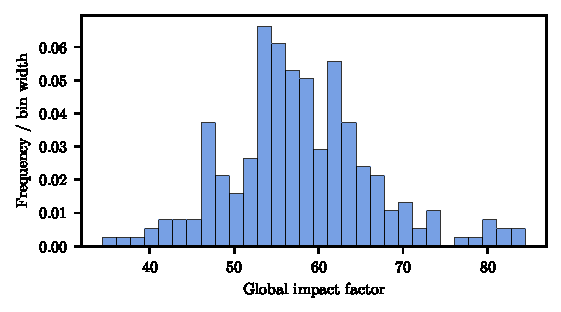
\includegraphics{IF-frequency.pdf}
		\caption{Frequency distribution of global impact factor}
		\label{fig:freqIF}
		\end{figure}
	
		{
			\fontsize{10}{14}\selectfont
			{
				\begin{longtable}{ccccccc}
					\caption{Descriptive statistics of the global impact factor}
					\label{tb:IFDistribution}\\
					
					\toprule
					Mean&Standard Deviation&Kurtosis&Skewness&Range&Median&Confidence Level (95.0\%)\\
					\toprule
					57.9&8.65&0.81&0.41&50.51&57.25&1.13\\
					\bottomrule
				\end{longtable}
			}
		}
		
		We draw a histogram by using 226 global factors IF$_G$ (see Fig.\ref{fig:freqIF}), and calculate several statistical characteristics for the distribution (see Table \ref{tb:IFDistribution}).  
		
		IF$_G$ is roughly concentrated around the mean and the median but does not exactly follow a normal distribution.  The distribution is skewed to the right according to the table, meaning that there is a longer left tail.  However, we can observe a right tail as well on the histogram.  Neither tail is very long.  There are no values below 30 or above 90.
		
	\subsubsection{Local Impact Factor Results}
		
		For calculating local impact factor IF$_L$:
		\vspace{-0.2cm}
		\begin{itemize}
		\item First, we chose 3 locations Florida (FL), Neveda (NV), and Alaska (AK), where Florida is warm and humid, Neveda is hot and dry, and Alaska is extremely cold;
		\vspace{-0.2cm}
		\item Then, we chose 5 plants that are invasive at these locations.  Sweetclover ranks the first in global impact factor; the tree of heaven is the highest ranking tree in terms of global impact factor; yellow salsify has the highest global impact factor among nontoxic plants; mugo pine is in the last place in the global impact table; also, dandelion is not left out.
		\vspace{-0.2cm}
		\item Last, we prepare all the attributes options with regards to \textbf{Category \textit{C}} and implement the model to get local impact factor IF$_L$.
		\end{itemize} 	
		
		The results are shown in Fig.\ref{fig:IFLocal}.  
		
		For each plant, their impact would be greater at locations with more favorable environments, and vice versa.
		
		For different plants, their local impact factor ranking roughly conforms to the global one, but there are exceptions.  For example, though sweetclover has a IF$_G$ higher than that of the tree of heaven, the IF$_L$ for sweetclover in Alaska is lower than that for the tree of heaven in Florida.
		
		\begin{figure}[htbp]
			\centering
			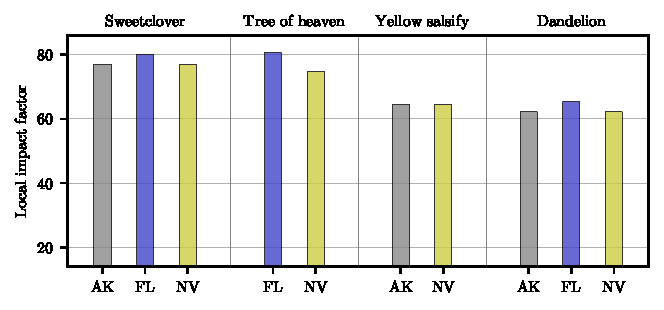
\includegraphics{IF_local-loc.pdf}
			\caption{Local impact factor}
			\label{fig:IFLocal}
		\end{figure}

	\newpage
	
	\subsection{Sensitivity Analysis}
	
		In \textbf{Eq.\ref{eq:ifg}} and Eq.\ref{eq:ifl}, the impact factors are evaluated as 100$\rho$ multiplied by a linear combination of attribute values.  We discuss the model's sensitivity as follows:
		\vspace{-0.2cm}
		\begin{itemize}
			\item For variable $\rho$, when other variables do not change, changing $\rho$ from 1.0 to 0.9 will lead to a 90\% discount to current \textbf{IF} value;
			\vspace{-0.2cm}
			\item For one certain attribute value, when other variables do not change, the change of impact factor is in proportion with the change of the attribute value.  The formula is as follows:
			\[
				\Delta\mathrm{IF} = 100\rho\cdot w\Delta v
			\]
			
			Where:
			
			{
			\setlength{\parindent}{2em}
			$\Delta\mathrm{IF}$ is the change of impact factor value;
			
			\vspace{-0.15cm}
			$\Delta v$ is the change of the attribute value;
			
			\vspace{-0.15cm}
			$w$ is the attribute weight corresponding to the attribute.
			}
			
			\vspace{0.15cm}
			
			For example, if only attribute $B_1$ (Toxicity) changes from ``None'' to ``Severe'', the change of attribute value $\Delta v$ equals 1 (Table \ref{tb:mat}).  Considering that the weight of $B_1$ for global impact factor is $\beta_1$ = 0.227 and for local impact factor is $\beta_1$ = 0.192 (Table \ref{tb:weights}), we will conclude that global impact factor will increase 22.7$\rho$ and local impact factor will increase 19.2$\rho$.
			
		\end{itemize} 
		
		
	\subsection{Strengths and Weaknesses}

		\paragraph{Strengths}
		\vspace{-0.1cm}
		\begin{itemize}
			\vspace{-0.3cm}
			\item Our model is \textbf{easy to implement}.  For one plant, we can design a questionnaire to collect its attribute options and use our model to calculate the impact factors quickly.
		\end{itemize}
		
		\paragraph{Weaknesses}
		\vspace{-0.5cm}
		\begin{itemize}
			\vspace{-0.3cm}
			\item Our model is \textbf{subjective}.  The weights are subjectively determined.  If we could involve experts or research results in determining the attribute weights, our model could be more accurate.
			
			\vspace{-0.2cm}
			\item Our attribute design may be \textbf{uncomprehensive}.  It is possible that we have overlooked some other important attributes.
		\end{itemize}

\newpage
\section*{\begin{center} Our Vigorous Friend \end{center}}
\addcontentsline{toc}{section}{Our Vigorous Friend}
\vspace{-1cm}
It is always a dreamlike scene to see the dandelion flying on a summer day.  All those little parachutes drift in the air, slowly and gently, through a beam of light, like angels from the sky.

We know how children love dandelions.  They never tire of blowing puffballs and running after the parachutes.  But we also know how adults dislike them.  The dandelions cause allergy, grow with our crops, and spread like mad.  Most of the time, we label them as invasive herbs that need great effort to take care of.

Whether we like them or not, dandelions spread all over the world.  They can adapt to almost all kinds of environments, regardless of what the soil quality, humidity and temperature are.  They grow fast, have abundant seeds and propagate without relying on other creatures.  They never tire of dispersing, germinating and flowering.  Looking at them, we have to admit they are so vigorous and full of vitality.

That is why they cannot stop ``invading''.  But we need to be aware that ``invasion'' should be a neutral word than a negative word for nature species.  When we talk about species invading, it should be no difference from talking about emergence, prosperity, mutation or even extinction of species.  These are all natural processes.  Study has proved that without human intervention, even invasive species can get to an equilibrium with other species.  At some points, the invasive species could develop very fast and occupy a lot of resources, but gradually, when other species go into competition sufficiently, all the species will get along in harmony and share our planet peacefully.

We believe it is the same for our human beings - we will get along well with all the species including invasive ones.

Sometimes it is we humans who flap the butterfly's wing.  The Brazilian red eared turtle was a hit in the pet market. However, some people purchased them and released them in the wild due to their compassion. Soon the turtles dominated the aquatic ecosystem with their tenacious vitality.  Humans bring species from here to there and artificially raise them.  Humans sometimes introduce species which do not bring harm initially but do eventually.  We humans break the balance of nature and make the whole ecological system blink.

The invasive species are just who they are.  Most of them have a lot of merits to human beings.  They can provide fodder for our livestock, or they can be food or medicine.  They are so lovely when we learn to get along with them.  Think about dandelions.  They have never been labeled invasive until recently.  But they have been evolving in this planet for about 30 million years! Long enough to prove their innocence.  It is not fair to treat them like an enemy.  They are just old friends, sometimes sweet, sometimes petulant, and after all they just very vigorous and full of vitality.  We are so lucky that they are around -- children will definitely agree with us, and how about adults?

\newpage

\begin{spacing}{0.9}
\phantomsection
\addcontentsline{toc}{section}{References}
\newrefcontext
\printbibliography
\end{spacing}
	
\end{document}
